% !TeX root = f61_longreport_schmitt_kleinbek.tex
\section{Measurements Log and Evaluation}



\subsection{Experimental setup}
The relaxation times and the chemical shift were measured with a Bruker minispec p20 (see fig. \ref{fig:setup}).
%\begin{figure}[ht]
%\centering
%\begin{subfigure}{.45\textwidth}
%\centering
%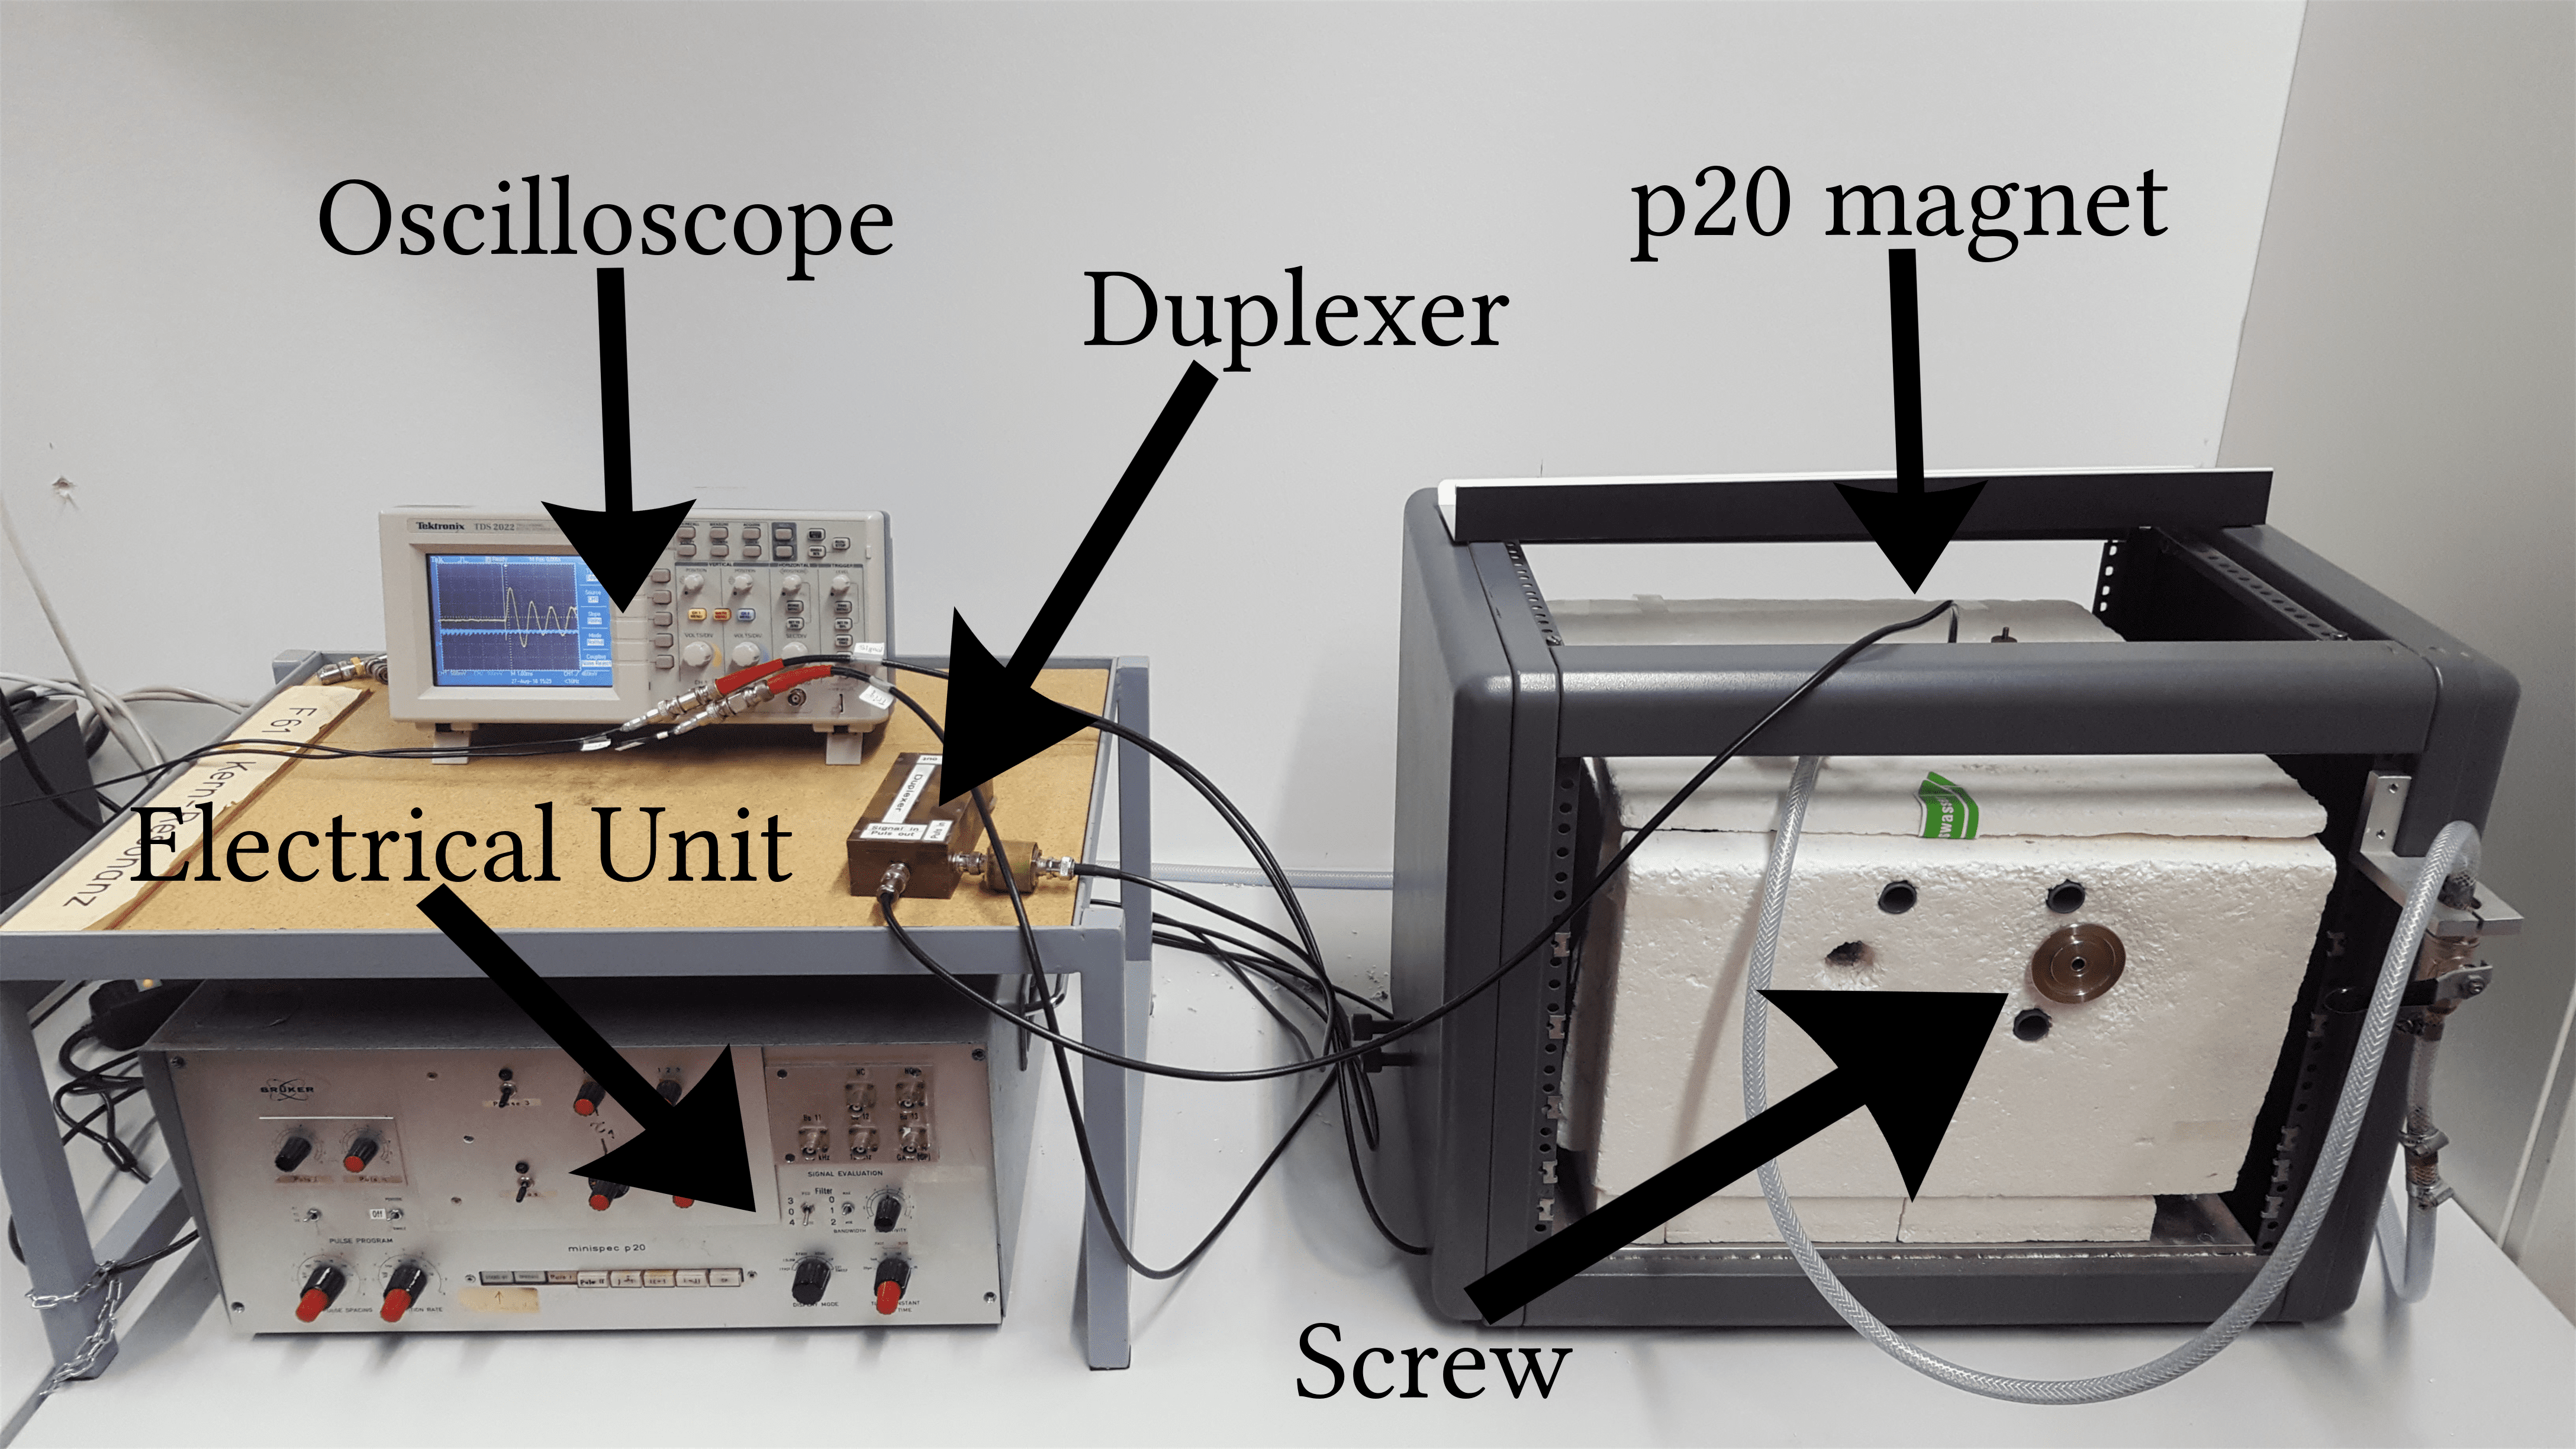
\includegraphics[height =4.5cm]{images//setup.png}
%\caption{Entire Configuration}
%\end{subfigure}
%\quad
%\begin{subfigure}{.45\textwidth}
%\centering
%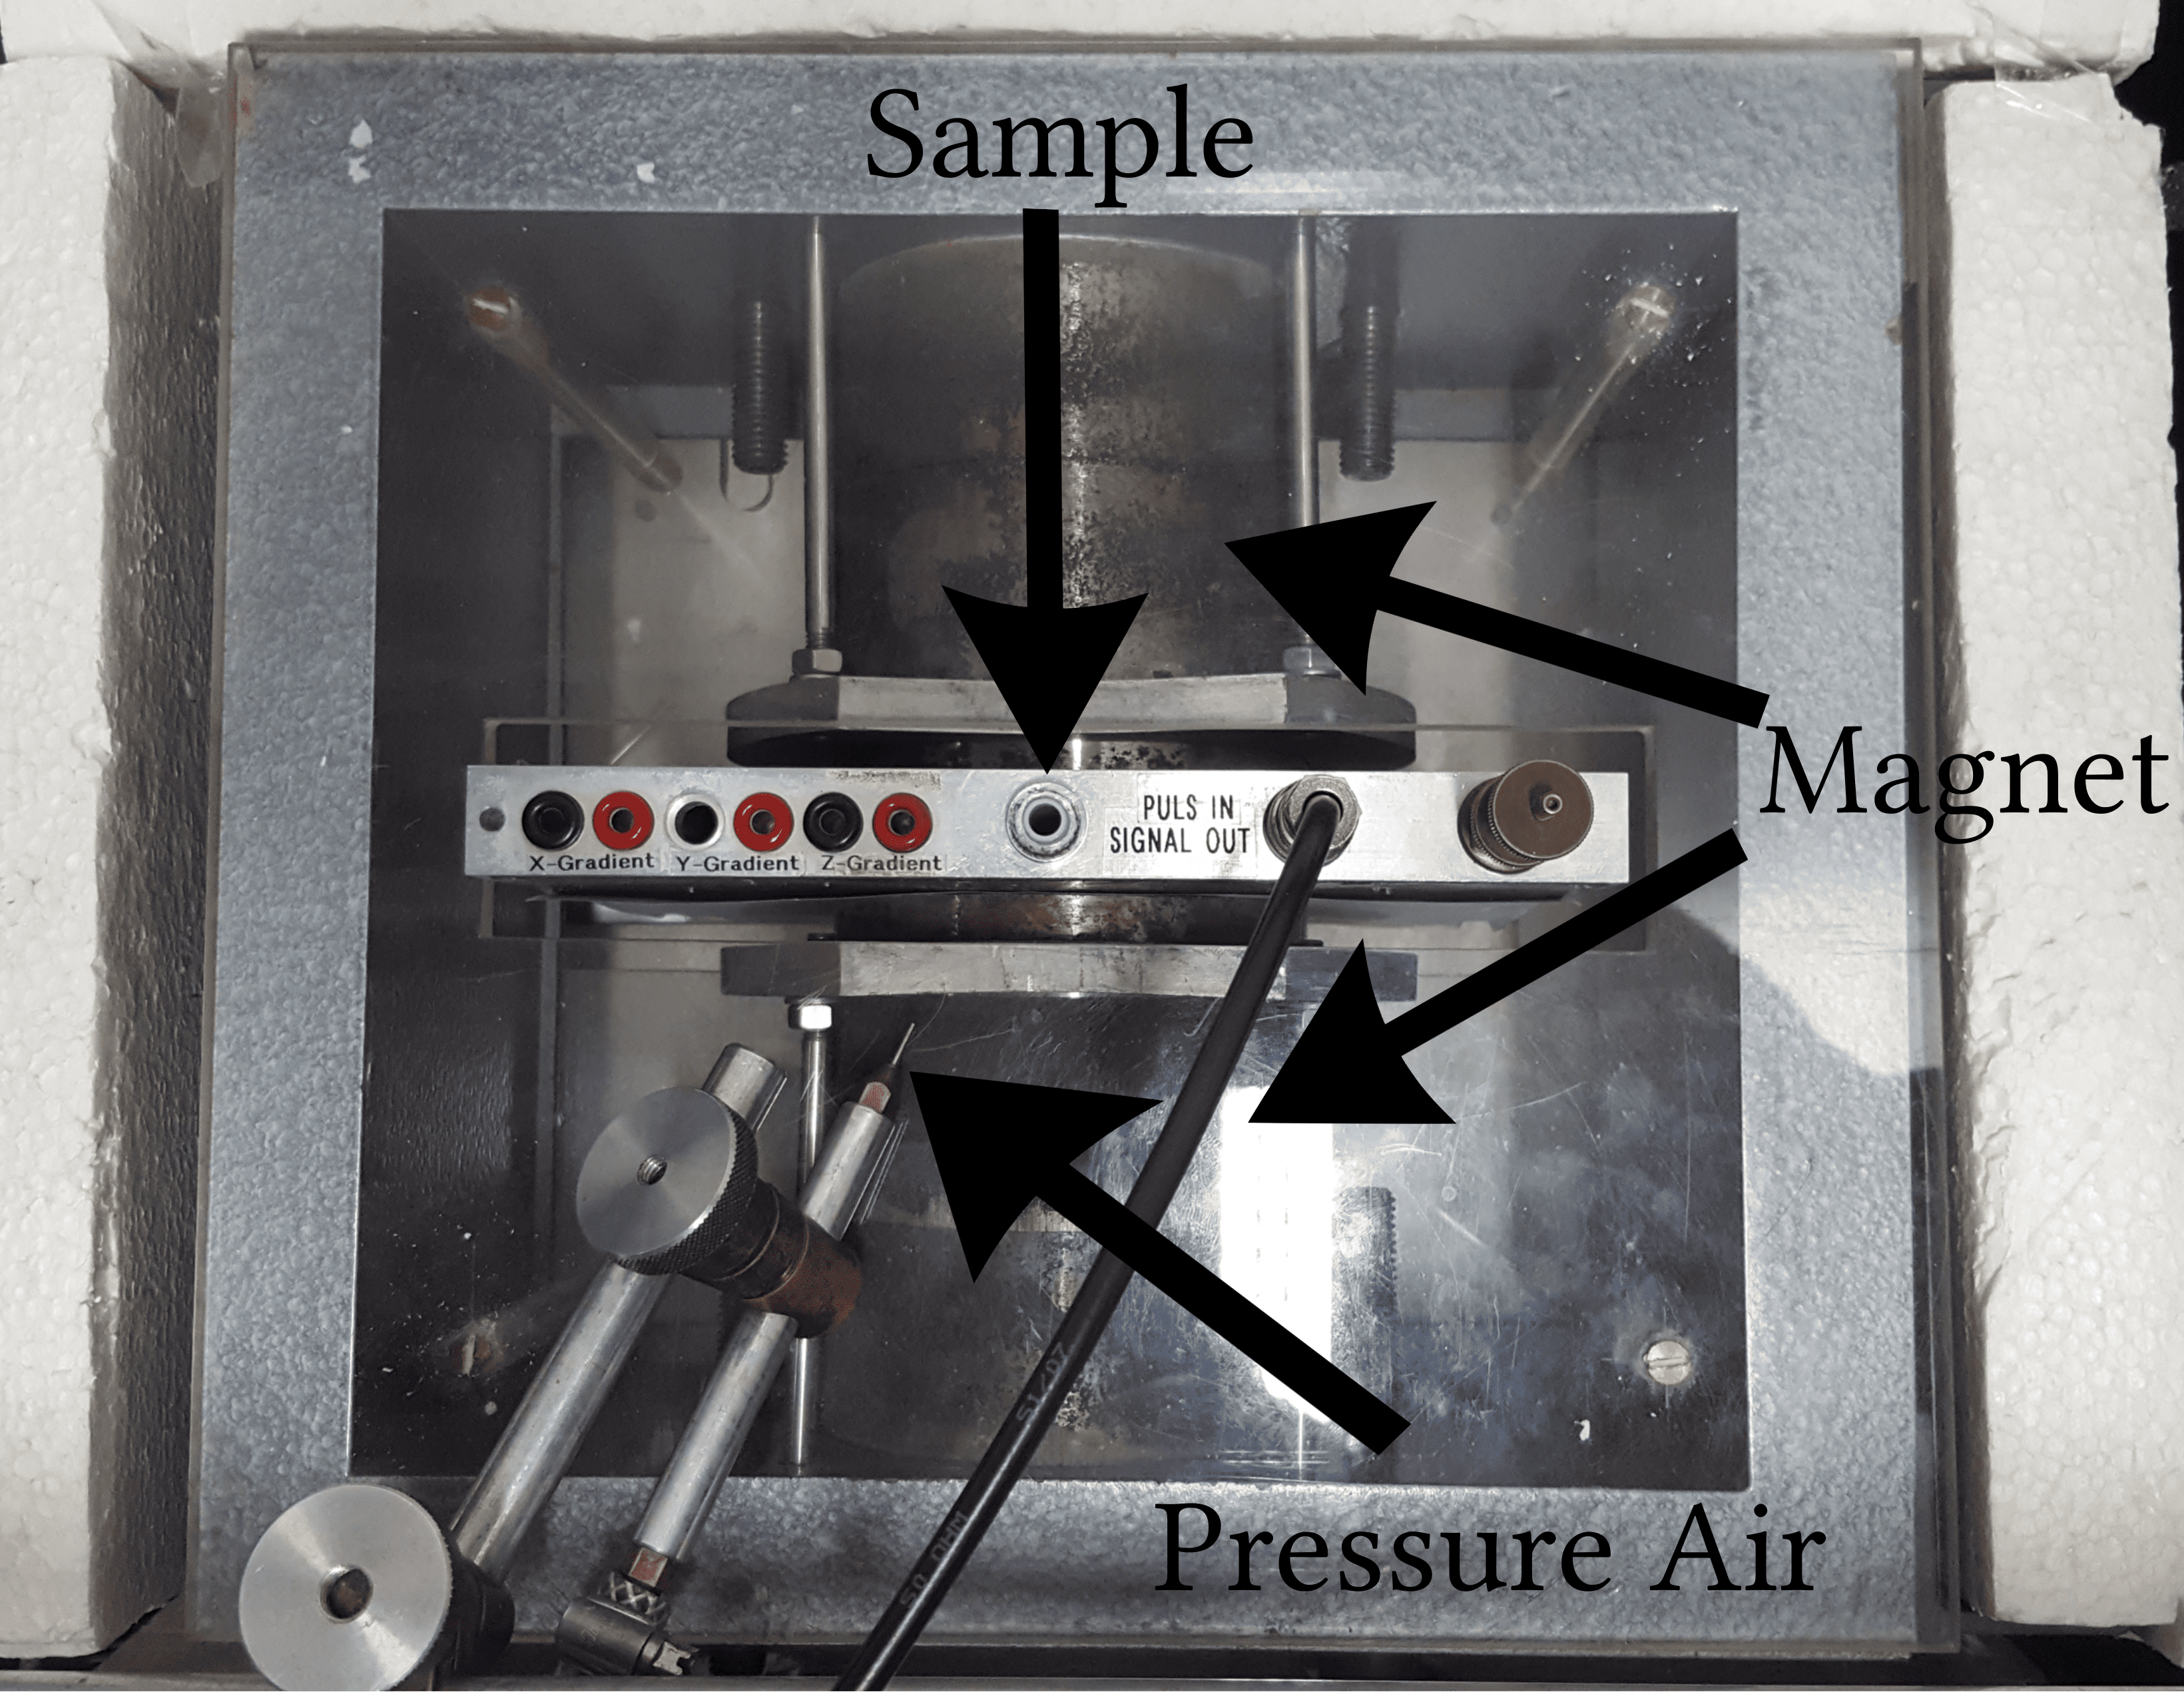
\includegraphics[height=4.5cm]{images//magnet.png}
%\caption{p20 magnet}
%\end{subfigure}
%\caption{Experimental setup}
%\end{figure}
The arrangement is divided into the p20 electrical unit and the p20 magnet.\\
The electrical unit can generate two different pulses (hereinafter called pulse I and pulse II), as well as I-I, I-II and II-I sequences and a Carr-Purcell sequence.
For the sequences the duration between the individual pulses and for the individual pulses the pulse duration can be set.
The latter was later adjusted so that the two pulses correspond to a $\ang{90}$ or $\ang{180}$ pulse.
The signal generated by the electrical unit is conducted into the magnet, where it generates a magnetic field that deflects the magnetic moments of the atomic nuclei in the sample.
These rotate as described in the previous section now with the Larmor frequency and generates a signal with this frequency in an induction coil inside the structure, which is fed back into the electronic unit via the duplexer, where it is modulated with the high-frequency excitation frequency.
The resulting signal has an operating frequency which indicates the difference between the excitation frequency and the Larmor frequency.
This is displayed on the oscilloscope and read out and evaluated on the PC with LabView.



\subsection{Determination of relaxation time}
\begin{table}[ht]
\centering
\begin{tabular}{cccc}
\toprule
Sample & $T_1$ [ms] & $T_{2,\text{ Spin-echo}}$ [ms] & $T_{2,\text{ Carr-purcell}}$ [ms]\\
\midrule
Gd500 & \num{190.0(6)} & \num{154.2(9)} & \num{170.1(4)}\\
Gd600 & \num{234.3(5)} & \num{186.5(9)} & \num{198.2(7)}\\
\bottomrule
\end{tabular}
\caption{Measured relaxation time}
\label{tab:relax}
\end{table}
\begin{figure}[ht]
\begin{subfigure}{.45\textwidth}
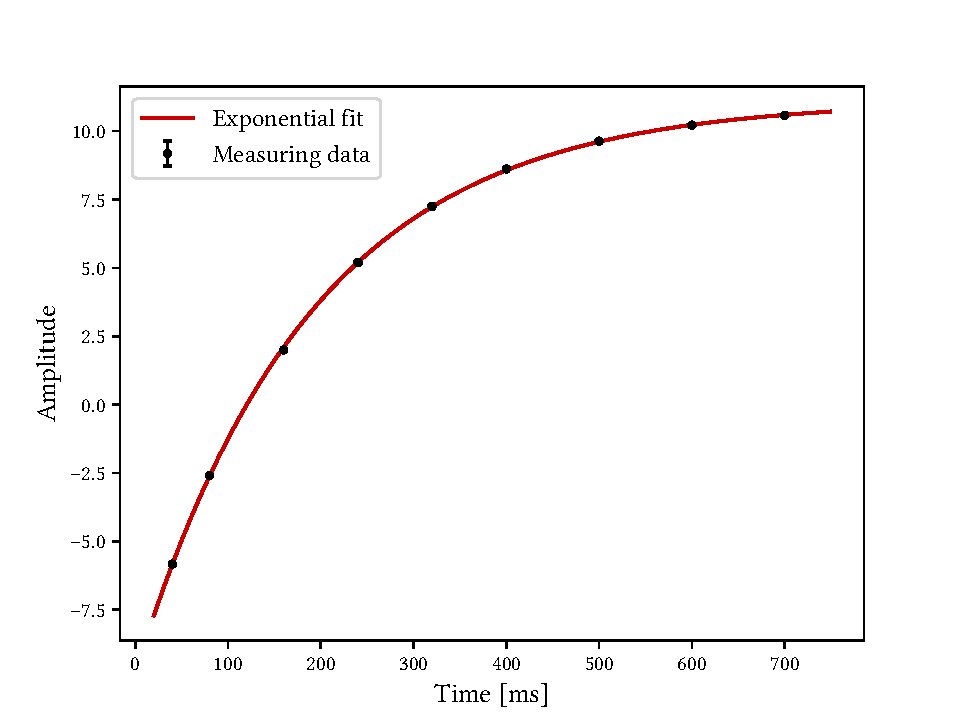
\includegraphics[width=9.3cm]{..//figures//f61_abb_1.pdf}
\caption{Gd500}
\end{subfigure}
\qquad
\begin{subfigure}{.45\textwidth}
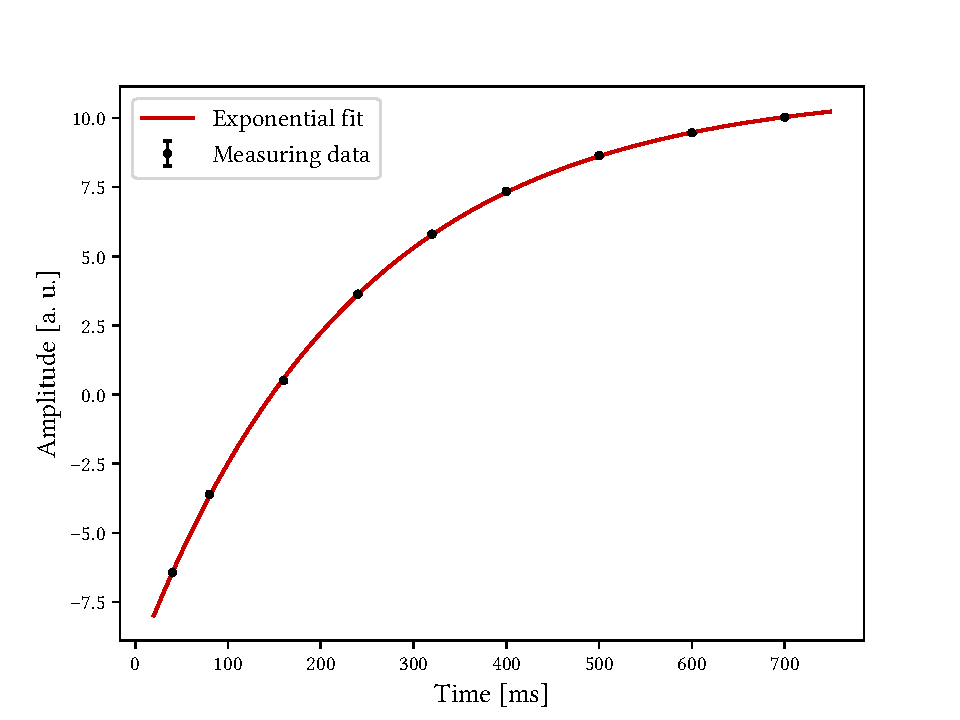
\includegraphics[width=9.3cm]{..//figures//f61_abb_1_600.pdf}
\caption{Gd600}
\end{subfigure}
\caption{Results of the measurement for relaxation time $T_1$}
\label{fig:t1}
\end{figure}

\begin{figure}[ht]
\begin{subfigure}{.45\textwidth}
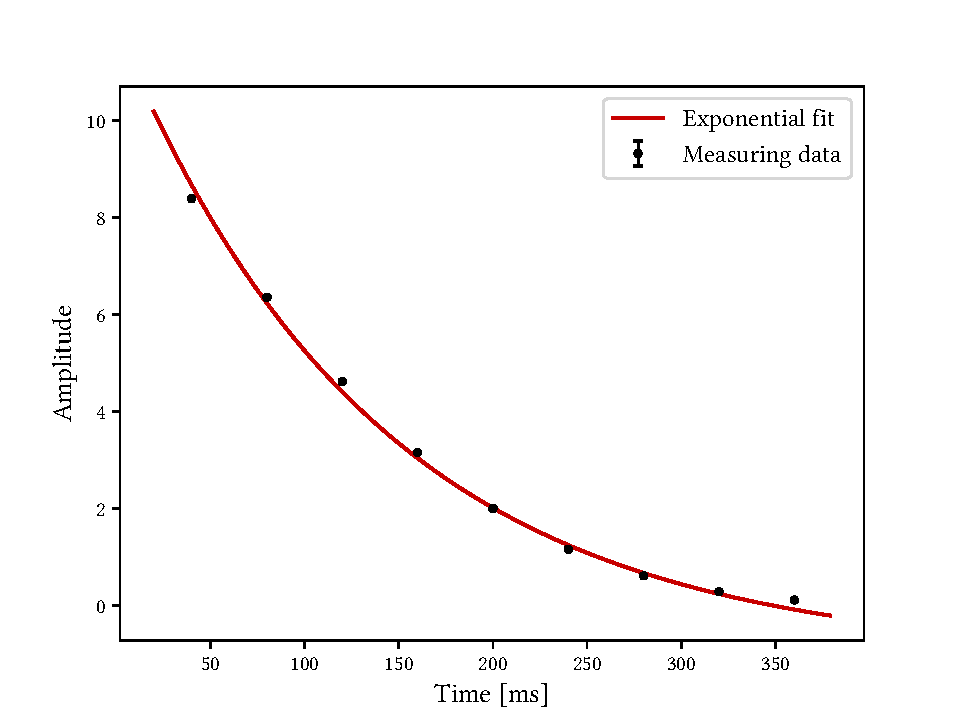
\includegraphics[width=9.3cm]{..//figures//f61_abb_2.pdf}
\caption{Gd500}
\end{subfigure}
\qquad
\begin{subfigure}{.45\textwidth}
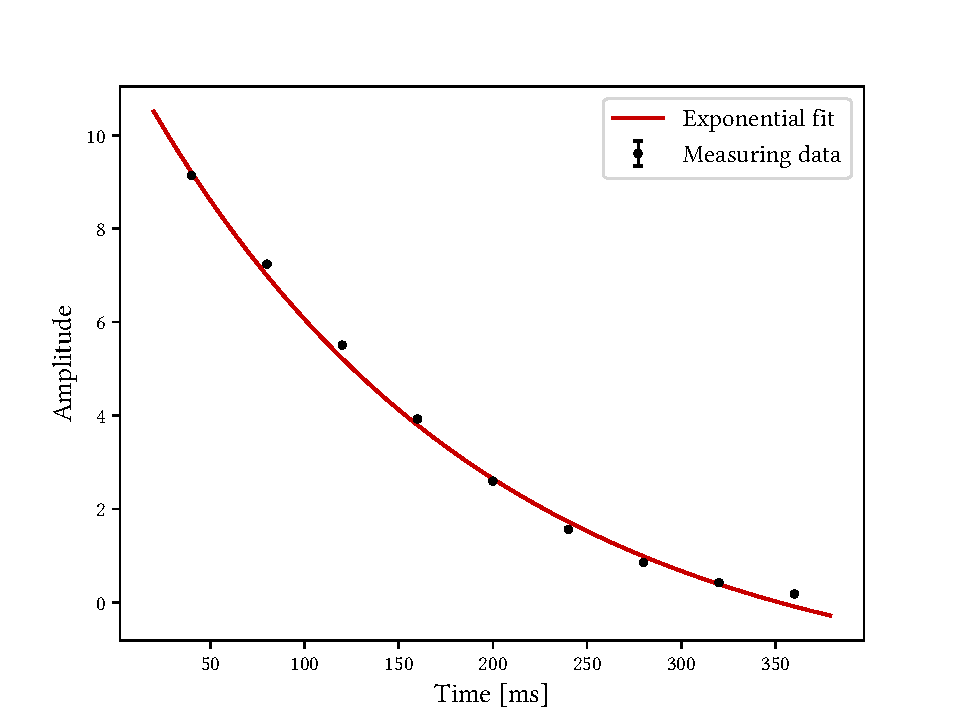
\includegraphics[width=9.3cm]{..//figures//f61_abb_2_600.pdf}
\caption{Gd600}
\end{subfigure}
\caption{Results of the measurement for relaxation time $T_2$ using spin-echo method}
\label{fig:t2se}
\end{figure}

\begin{figure}[ht]
\begin{subfigure}{.45\textwidth}
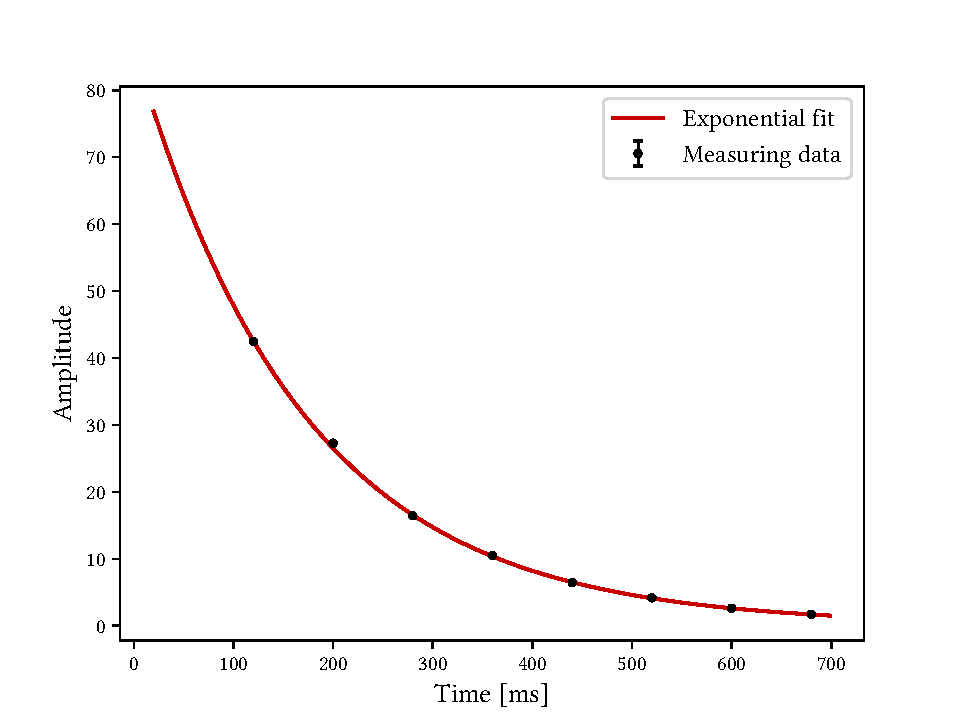
\includegraphics[width=9.3cm]{..//figures//f61_abb_3.pdf}
\caption{Gd500}
\end{subfigure}
\qquad
\begin{subfigure}{.45\textwidth}
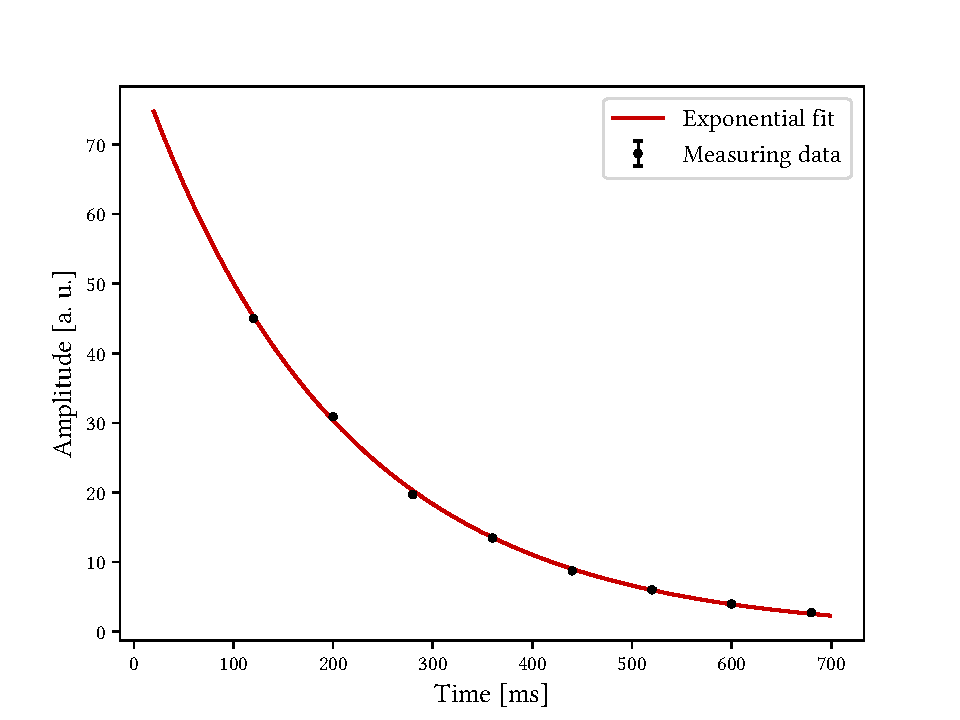
\includegraphics[width=9.3cm]{..//figures//f61_abb_3_600.pdf}
\caption{Gd600}
\end{subfigure}
\caption{Results of the measurement for relaxation time $T_2$ using Carr-purcell sequence}
\label{fig:t2cp}
\end{figure}



\subsection{Chemical shift}
In this part of the experiment we measured the Larmor frequencies of unknown substances with and without the reference substance TMS.
This was done by measuring the resonance peaks of the Fourier transform of the registered signal.
\begin{figure}[ht]
\begin{subfigure}{.45\textwidth}
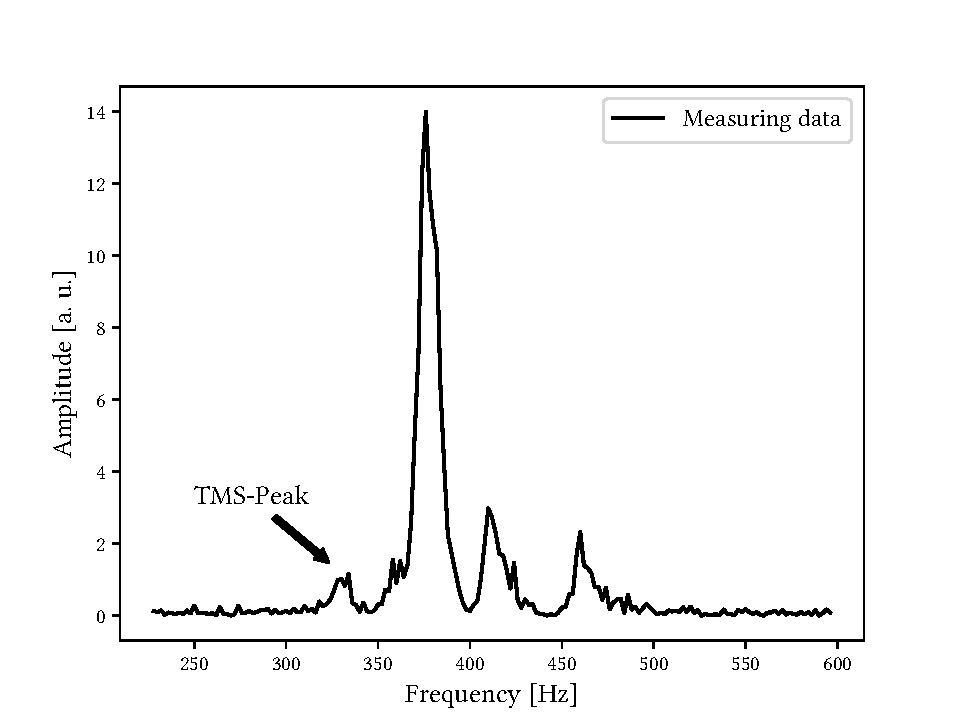
\includegraphics[width=9.3cm]{..//figures//f61_abb_4.pdf}
\caption{Sample A}
\end{subfigure}
\qquad
\begin{subfigure}{.495\textwidth}
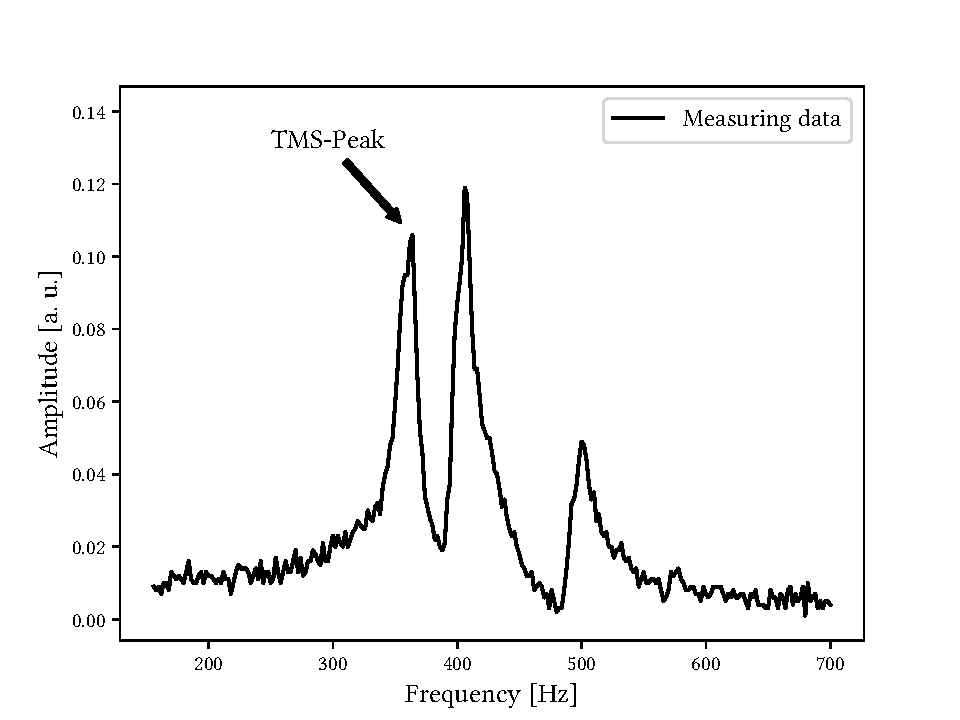
\includegraphics[width=9.3cm]{..//figures//f61_abb_5.pdf}
\caption{Sample B}
\end{subfigure}
\qquad
\begin{subfigure}{.45\textwidth}
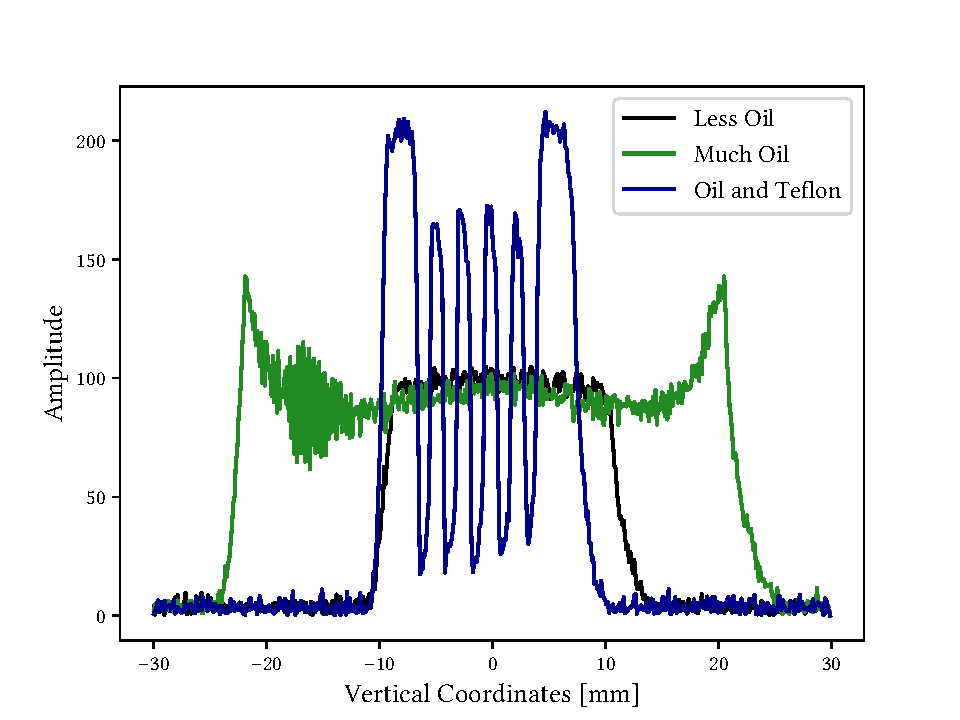
\includegraphics[width=9.3cm]{..//figures//f61_abb_6.pdf}
\caption{Sample C}
\end{subfigure}
\qquad
\begin{subfigure}{.45\textwidth}
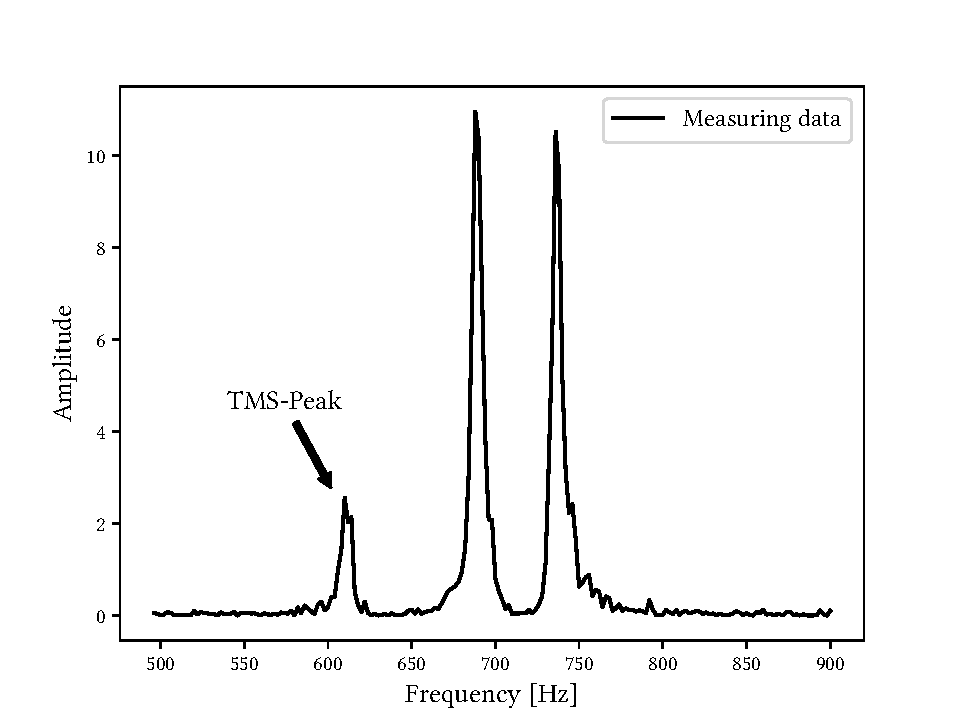
\includegraphics[width=9.3cm]{..//figures//f61_abb_7.pdf}
\caption{Sample D}
\end{subfigure}
\caption{Fourier transform of the registered signal}
\label{fig:fourier}
\end{figure}
From the frequency shift measured in this way, the chemical shift can be calculated using equation \ref{eq:shift}.\\
Experimentally, we had to give a pulse to the magnet every three seconds and continuously adjust the main magnetic field so that the working frequency is around $\nu_\text{w}=\SI{500}{\hertz}$.
Therefore, one wavelength had to be \SI{2}{\milli\second} long, which we could achieve via the screw on the magnet.\\
Table \ref{tab:shift} lists the measured chemical shifts of the different samples and their assignment to the corresponding chemical elements.
\begin{table}[ht]
\centering
\begin{tabular}{cccccc}
\toprule
Sample & Shift 1 [ppm] & Shift 2 [ppm] & Shift 3 [ppm] & Substance\\
\midrule
A & \num{2.4(1)} & \num{3.9(1)} & \num{6.3(1)} & fluoroacetone\\
B & \num{2.1(1)} & \num{6.9(1)} & & p-xylol\\
C & \num{9.6(1)} & \num{12.0(1)} & & acetic acid\\
D & \num{4.0(1)} & \num{6.4(1)} & & fluoroacetonitril\\
E & \num{2.2(1)} & \num{7.3(1)} & & tuluol\\
\bottomrule
\end{tabular}
\caption{Measured chemical shifts}
\label{tab:shift}
\end{table}
Due to missing samples A,D and E, the shifts could unfortunately only be taken over by leading test participants.\\

Now we knew that the elements toluol (CH$_3$ - C$_6$H$_5$), p-xylol (CH$_3$ - C$_6$H$_4$ - CH$_3$), acetic acid (CH$_3$ - COOH), fluoroacetone (FCH$_2$ - CO - CH$_3$) and fluoroacetonitril (FCH$_2$ - CN) were among the samples and could classify them according to the same principle with figure \ref{fig:shift}.\\
Sample C is the only one that has a shift above 10 ppm and therefore must have a COOH group, which only applies to acetic acid.
The two shifts of samples B and E are in fact the same.
The same functional groups, a carbon ring and one or two methyl groups for tuluol and p-xylol, cause the same shifts.
Because p-xylol contains twice the amount of methyl groups, this substance should show a higher ratio in the peak heights.
Sample B shows exactly such a difference and is therefore p-xylol, while sample E is then tuluol.
Both fluoroacetone and fluoroacetonitril have a fluoromethyl group and show two identical shifts.
Nevertheless, the former has a third shift exactly the same size as tuluol and p-xylol, which could be assigned to the simple methyl group.
Therefore, sample A with the additional peak corresponds to fluoroacetone and sample D to fluoroacetonitril.



\subsection{Imaging techniques}
\subsubsection{One dimensional imaging}

\subsubsection{Two dimensional imaging}
\begin{figure}[ht]
\begin{subfigure}{.3\textwidth}
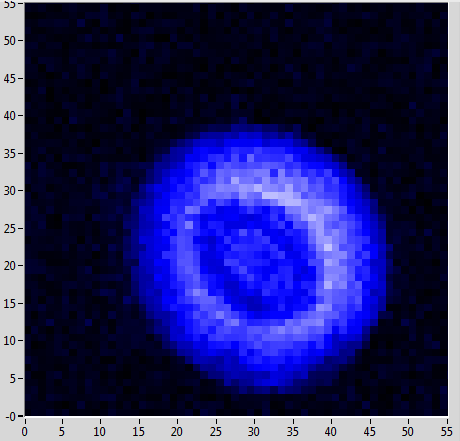
\includegraphics[width=5cm]{..//figures//olive.png}
\caption{Olive}
\end{subfigure}
\qquad
\begin{subfigure}{.3\textwidth}
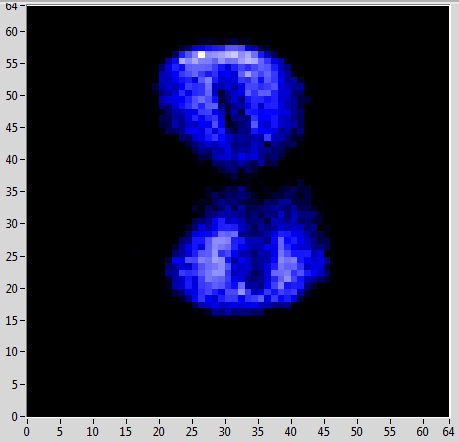
\includegraphics[width=5cm]{..//figures//peanut.png}
\caption{Peanut}
\end{subfigure}
\qquad
\begin{subfigure}{.3\textwidth}
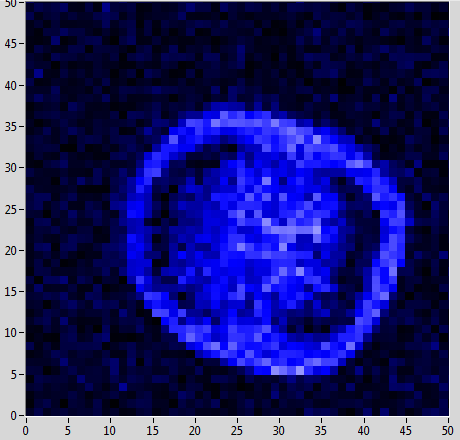
\includegraphics[width=5cm]{..//figures//chilipepper.png}
\caption{Chilipepper}
\end{subfigure}
\caption{Two dimensional NMR imaging}
\label{fig:2d}
\end{figure}